\chapter{ Der Weg zum Lichtquant}\index{Lichtquant}\index{Photon}\index{Licht}\index{Quantenphysik}\index{Quantenmechanik}

\setcounter{section}{2}
\setcounter{subsection}{0}
\setcounter{subsubsection}{1}
\setcounter{secnumdepth}{3}
% Boxen-Stile definieren
\tcbset{physikbox/.style={colback=blue!5!white, colframe=blue!75!black, fonttitle=\bfseries}}
\tcbset{mathebox/.style={colback=green!5!white, colframe=green!50!black, fonttitle=\bfseries}}
\tcbset{didaktikbox/.style={colback=yellow!5!white, colframe=yellow!50!black, fonttitle=\bfseries}}
\tcbset{hypobox/.style={colback=orange!5!white, colframe=orange!75!black, fonttitle=\bfseries}}
\tcbset{hinweisbox/.style={colback=gray!10!white, colframe=black!40!black, fonttitle=\bfseries}}

\subsection{Die klassische Lichttheorie und ihre Grenzen}\index{Klassische Physik}\index{Lichttheorie}

Die klassische Physik entwickelte im Laufe der Jahrhunderte zwei grundlegende Modelle zur Beschreibung des Lichts: das Teilchenmodell und das Wellenmodell.\index{Teilchenmodell}\index{Wellenmodell} Beide Modelle lieferten überzeugende Erklärungen für verschiedene Phänomene, stießen jedoch an fundamentale Grenzen, die zur Entwicklung der Quantentheorie führten.\index{Quantentheorie}

\subsubsection{Newtons Teilchentheorie des Lichts}
Isaac Newton\index{Newton, Isaac} ging davon aus, dass Licht aus winzigen Teilchen – sogenannten \emph{Korpuskeln} – bestehe, die sich geradlinig ausbreiten. Dieses Modell konnte die Reflexion und die geradlinige Ausbreitung gut erklären, versagte jedoch bei Phänomenen wie Beugung oder Interferenz.\index{Beugung}\index{Interferenz}
% In der Präambel (falls noch nicht vorhanden):
%\AtBeginEnvironment{tcolorbox}{\pretocmd{\tcbtitletext}{\ignorespaces}{}{}}
\vspace{1em}
% Im Dokument:
\begin{tcolorbox}[physikbox, title=Isaac Newton(1704) Teilchentheorie\textit{ \cite{newton_opticks}}]
	\label{box:newton}
	
	\emph{„Are not the rays of light very small bodies emitted from shining substances?“}
	
	\vspace{6pt}
	\textbf{Kommentar:} Newton formulierte die erste systematische Teilchentheorie des Lichts. Obwohl sein Modell viele Phänomene erklären konnte, scheiterte es an Beugung und Interferenz – was später zur Entwicklung der Wellentheorie führte.
\end{tcolorbox}
\index{Teilchentheorie des Lichts}
\subsubsection{Huygens’ Wellenmodell}
Christiaan Huygens\index{Huygens, Christiaan} stellte dem ein Wellenmodell gegenüber, in dem sich Licht als Ausbreitung von Wellenfronten in einem hypothetischen Medium, dem \emph{Äther}, bewegt.\index{Äther} Dieses Modell konnte Phänomene wie Interferenz und Beugung erfolgreich beschreiben, insbesondere nach Youngs Doppelspalt-Experiment (1801).\index{Doppelspalt}
\vspace{1em}
\begin{tcolorbox}[physikbox, title={Huygens (1960) über Lichtausbreitung \cite{huygens_light}}]
	\label{box:huygens}
	“Light is produced by a very small agitation of the ether and spreads successively.”\\
	
	
	\vspace{1em}
	
	\textbf{Kommentar:} Huygens entwickelte ein konsistentes Wellenmodell des Lichts, bei dem sich Licht als mechanische Schwingung im Äther ausbreitet – ähnlich dem Schall in der Luft. Diese Theorie war richtungsweisend für die Erklärung von Brechung und Interferenz, auch wenn die Existenz des Äthers später widerlegt wurde.
\end{tcolorbox}
\vspace{1em}
\index{Wellenmodell}
\newpage
\noindent
\subsubsection{Maxwells Elektrodynamik}
Ein Meilenstein war James Clerk Maxwells\index{Maxwell, James Clerk} Theorie der Elektrodynamik (1865).\index{Elektrodynamik} Sie vereinte Elektrizität und Magnetismus zu einer einheitlichen Theorie und zeigte, dass sich elektromagnetische Wellen mit Lichtgeschwindigkeit ausbreiten – ein Durchbruch, der Licht als elektromagnetische Welle erklärte.\index{Elektromagnetische Welle} Die Wellennatur des Lichts war damit in der klassischen Physik fest verankert.
	\vspace{1em}
\begin{tcolorbox}[physikbox,title={Maxwell (1873)über Licht und elektromagnetische Wellen \cite{maxwell_treatise}}]
	\label{box:maxwell}
	“The agreement of the results seems to show that light and magnetism are affections of the same substance, and that light is an electromagnetic disturbance propagated through the field according to electromagnetic laws.”\\
	
	
	\vspace{1em}
	
	\textbf{Kommentar:} Maxwell verknüpfte erstmals Licht mit dem elektromagnetischen Feld.\index{Elektromagnetisches Feld} In seinen Gleichungen erscheint Licht nicht mehr als mechanische Bewegung eines Äthers, sondern als selbständige elektromagnetische Welle, die sich mit endlicher Geschwindigkeit durch den Raum ausbreitet. Damit legte er den Grundstein für ein neues Verständnis der Lichtausbreitung ohne materielles Trägermedium.
\end{tcolorbox}

\subsubsection{Grenzen der klassischen Theorie}
Trotz ihrer Erfolge stieß die klassische Lichttheorie gegen Ende des 19. Jahrhunderts an schwerwiegende Grenzen:

\begin{itemize}
	\item \textbf{Schwarzkörperstrahlung:}\index{Schwarzkörperstrahlung} Die klassische Theorie sagte eine unendliche Energieabstrahlung bei hohen Frequenzen voraus (\emph{Ultraviolett-Katastrophe}).\index{Ultraviolett-Katastrophe}
	\item \textbf{Photoelektrischer Effekt:}\index{Photoeffekt} Die beobachteten Ergebnisse (z.\,B. frequenzabhängige Elektronenemission) widersprachen den Vorhersagen der klassischen Theorie.
	\item \textbf{Compton-Effekt:}\index{Compton-Effekt} Die Streuung von Röntgenstrahlung an Elektronen ließ sich nur mit Teilchenimpuls erklären.
\end{itemize}

Diese Widersprüche markierten eine fundamentale Krise der klassischen Physik und leiteten den Paradigmenwechsel zur Quantentheorie ein, bei dem das Licht sowohl Teilchen- als auch Welleneigenschaften besitzt.

\subsection{Die Schwarzkörperstrahlung}\index{Schwarzer Körper}

\subsubsection{Einleitung}
Die Schwarzkörperstrahlung zählt zu den Phänomenen, die das klassische Weltbild der Physik ins Wanken brachten. Zwar konnte man das von erhitzten Körpern ausgesandte Strahlungsspektrum präzise messen, doch alle klassischen Theorien versagten bei seiner Erklärung. Besonders im kurzwelligen Bereich führten die Gleichungen zu unphysikalischen Vorhersagen: einer unendlichen Energiedichte – bekannt als \emph{Ultraviolett-Katastrophe}.\index{Ultraviolett-Katastrophe}

Dieser fundamentale Widerspruch zwischen Theorie und Experiment zwang die Physik zu einem radikalen Umdenken. Erst Max Plancks\index{Planck, Max} Annahme, dass Energie nur in diskreten Portionen – sogenannten Quanten – abgegeben wird, führte zu einer Formel, die das beobachtete Spektrum korrekt beschreiben konnte. Damit war der Grundstein für die Quantentheorie gelegt.

\subsubsection{Was ist ein Schwarzer Körper?}

Ein \emph{Schwarzer Körper} ist ein ideales physikalisches Objekt, das sämtliche auftreffende elektromagnetische Strahlung vollständig absorbiert – unabhängig von Wellenlänge und Einfallsrichtung. Im thermischen Gleichgewicht gibt ein solcher Körper Strahlung ab, die nur von seiner Temperatur abhängt und ein charakteristisches Spektrum besitzt: die sogenannte \emph{Schwarzkörperstrahlung}.

Ein perfekter Schwarzer Körper reflektiert keinerlei Licht – er erscheint daher bei Zimmertemperatur vollkommen schwarz. In der Realität lassen sich solche Körper nur annähern, beispielsweise durch eine Hohlkugel mit kleiner Öffnung: Strahlung, die einmal ins Innere gelangt, wird vielfach reflektiert und nahezu vollständig absorbiert.

Die thermische Strahlung eines Schwarzen Körpers ist universell: Sie hängt nicht von Material oder Form ab, sondern nur von der Temperatur. Sie stellt damit ein zentrales Referenzmodell in der Thermodynamik und Strahlungsphysik dar.\index{Thermodynamik}\index{Strahlungsphysik}
\newpage
\noindent
\vspace{1em}
\begin{tcolorbox}[colback=blue!5!white, colframe=blue!50!black, title=Was ist ein schwarzer Körper?]
	\label{box:schwarzerkoerper}
	Ein schwarzer Körper ist ein ideales physikalisches Modell:
	
	\begin{itemize}
		\item Er absorbiert sämtliche einfallende elektromagnetische Strahlung – unabhängig von Frequenz oder Einfallswinkel.
		\item Die Strahlung, die er abgibt, hängt ausschließlich von seiner Temperatur ab – nicht von seiner Zusammensetzung.
		\item Die Spektralverteilung folgt dem Planckschen Strahlungsgesetz und zeigt ein Maximum, das sich mit der Temperatur verschiebt (Wiensches Verschiebungsgesetz).
	\end{itemize}
	
	Solche Modelle werden verwendet, um Wärmestrahlung von Sternen, Glühdrähten oder Hohlraumstrahlern zu beschreiben.
\end{tcolorbox}
\index{Plancksches Strahlungsgesetz}\index{Wiensches Verschiebungsgesetz}

\begin{figure}[H]
	\centering
	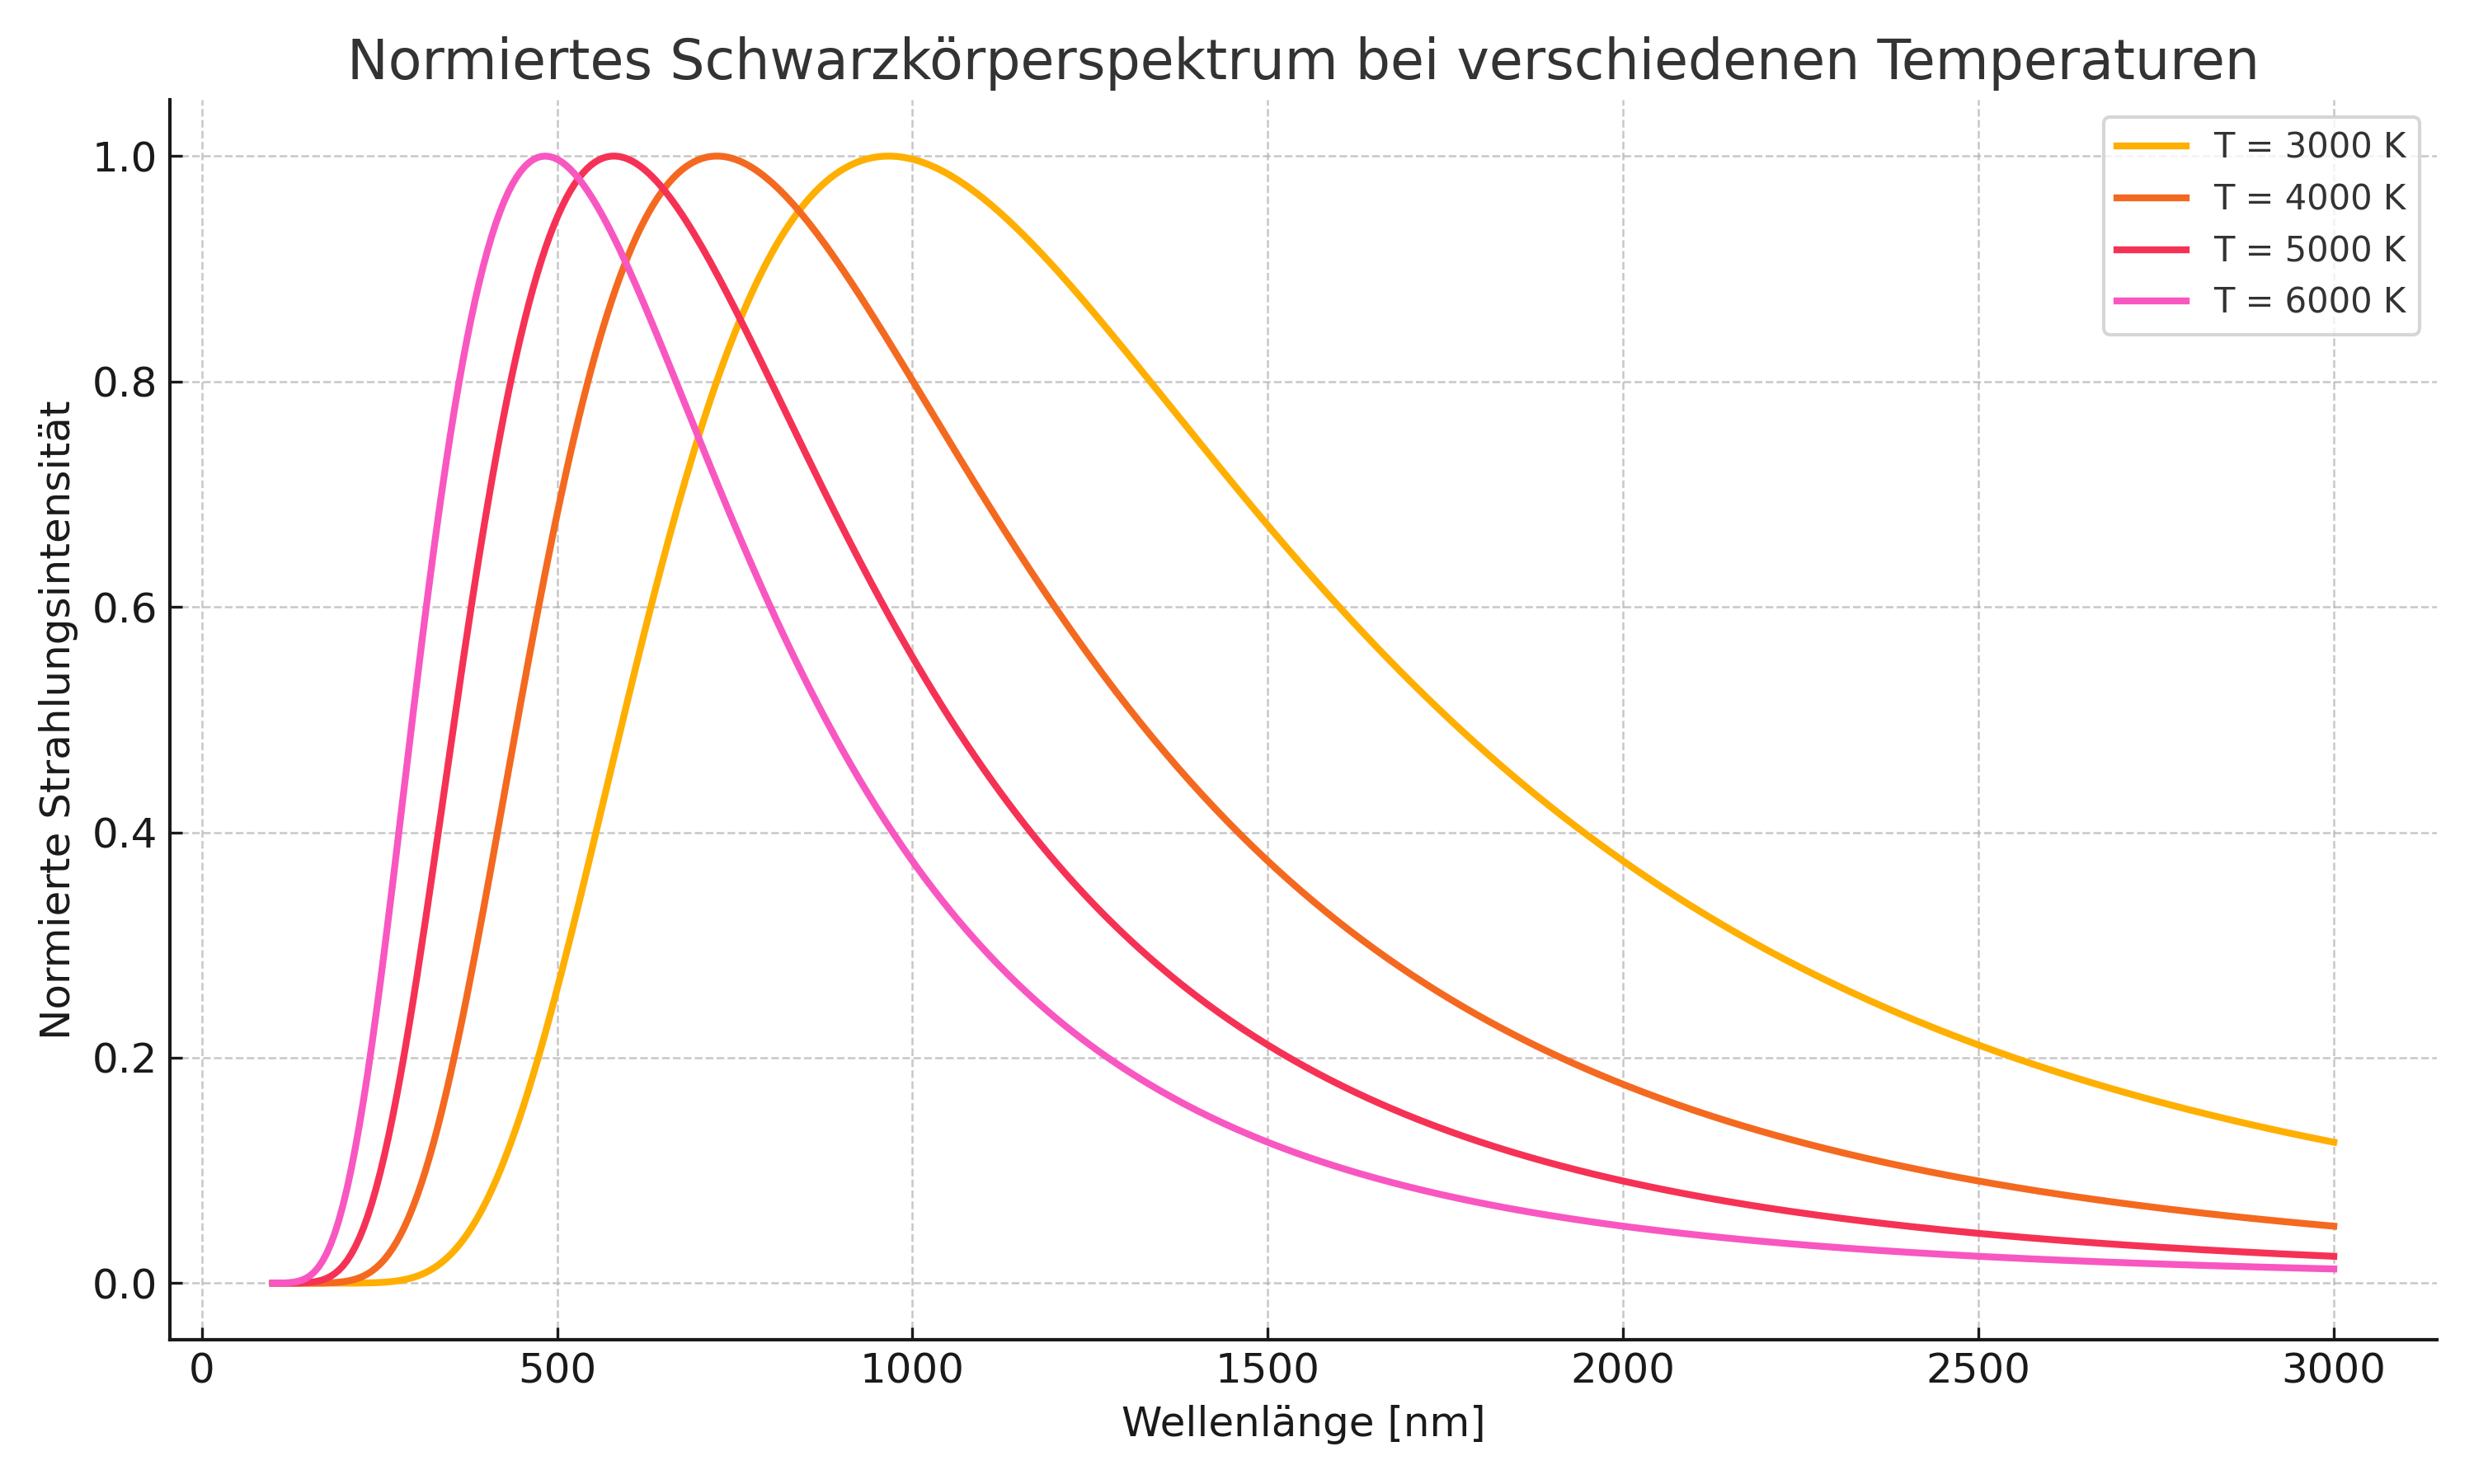
\includegraphics[width=0.85\textwidth]{bilder/schwarzer_koerper_spektrum.png}
	\caption{Normiertes Schwarzkörperspektrum für verschiedene Temperaturen. Das Maximum verschiebt sich mit zunehmender Temperatur zu kürzeren Wellenlängen (Wiensches Verschiebungsgesetz).}
	\label{fig:schwarzerkoerper}
\end{figure}

\subsubsection{Ablauf des Hohlraumexperiments}

Zur experimentellen Untersuchung der thermischen Strahlung verwendet man sogenannte \emph{Hohlraumstrahler}.\index{Hohlraumstrahler} Sie dienen als nahezu ideale Realisierung eines Schwarzen Körpers. Die typische Anordnung besteht aus einem massiven Metallblock mit einem inneren Hohlraum und einer kleinen Öffnung zur Außenwelt.
Strahlung, die durch diese Öffnung in das Innere gelangt, wird dort vielfach an den Wänden reflektiert und nahezu vollständig absorbiert. Umgekehrt tritt aus der Öffnung ein winziger Teil der inneren Gleichgewichtsstrahlung aus – diese entspricht nahezu exakt der theoretischen Schwarzkörperstrahlung bei der Temperatur \( T \) des Blocks.
Die aus der Öffnung austretende Strahlung wird mit einem Spektrometer untersucht.\index{Spektrometer} Dabei zeigt sich das typische Schwarzkörperspektrum: ein intensitätsabhängiger Verlauf mit einem Maximum, das sich mit der Temperatur verschiebt (Wiensches Verschiebungsgesetz), und ein charakteristischer Abfall im UV-Bereich. Diese Ergebnisse widersprachen der klassischen Physik fundamental und führten letztlich zur Entwicklung der Quantentheorie.

\begin{figure}[H]
	\centering
	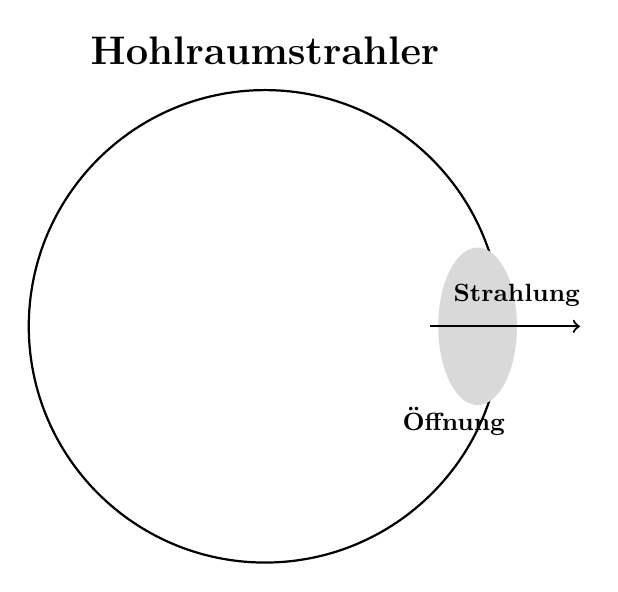
\begin{tikzpicture}
		% Hohlkörper
		\draw[thick] (0,0) circle(3);
		% Öffnung (rechts)
		\fill[gray!30] (2.7,0) ellipse (0.5 and 1.0);
		% Austretende Strahlung
		\draw[->, thick] (2.1,0) -- (4,0);
		\node at (3.2,0.4) {\small \textbf{Strahlung}};
		% Labels
		\node at (2.4,-1.2) {\small \textbf{Öffnung}};
		\node at (0,3.5) {\Large \textbf{Hohlraumstrahler}};
	\end{tikzpicture}
	\caption{Modell eines Hohlraumstrahlers zur Erzeugung nahezu idealer Schwarzkörperstrahlung.}
\end{figure}
\newpage
\noindent
\subsection{Versagen der klassischen Theorie – \newline das Rayleigh-Jeans-Gesetz}\index{Rayleigh-Jeans-Gesetz}

Im 19. Jahrhundert versuchten Lord Rayleigh und Sir James Jeans,\index{Rayleigh, Lord}\index{Jeans, James} die Schwarzkörperstrahlung mithilfe der klassischen Elektrodynamik und der statistischen Mechanik zu beschreiben.\index{Statistische Mechanik} Sie betrachteten stehende elektromagnetische Wellen in einem Hohlraum als harmonische Oszillatoren und berechneten die Energieverteilung durch Anwendung des Ausrüstungsprinzips der klassischen Thermodynamik.\index{Ausrüstungsprinzip}

Das Ergebnis war das sogenannte \emph{Rayleigh-Jeans-Gesetz}, das die spektrale Energiedichte in Abhängigkeit von der Wellenlänge \( \lambda \) und der Temperatur \( T \) beschreibt:

\[
u(\lambda, T) = \frac{8 \pi k T}{\lambda^4}
\]

Hierbei ist:
\begin{itemize}
	\item \( u(\lambda, T) \) die Strahlungsenergie pro Wellenlängenintervall und Volumen,
	\item \( k \) die Boltzmann-Konstante,\index{Boltzmann-Konstante}
	\item \( T \) die absolute Temperatur.
\end{itemize}

Für lange Wellenlängen liefert die Formel sinnvolle Ergebnisse und stimmt gut mit den experimentellen Daten überein. Doch bei kurzen Wellenlängen divergiert der Ausdruck gegen unendlich – es ergibt sich eine unphysikalische, unendliche Energiedichte:

\[
\lim_{\lambda \to 0} u(\lambda, T) \to \infty
\]

Dieses Problem wurde als \emph{Ultraviolett-Katastrophe} bekannt.\index{Ultraviolett-Katastrophe} Es widersprach fundamental den experimentellen Beobachtungen (siehe Abb.~\ref{fig:schwarzerkoerper}), bei denen die Strahlung im UV-Bereich keineswegs zunimmt, sondern stark abfällt.

Diese Katastrophe offenbarte die Grenzen der klassischen Physik. Eine neue Idee war erforderlich, um die Beobachtungen zu erklären – sie kam von Max Planck.
(Der Rechenweg über Modenzählung im Hohlraum und das klassische Ausrüstungsprinzip ist in Anhang~A, Abschnitt~\ref{anhangA:rayleigh} dargestellt.)
\subsection{Versagen der klassischen Theorie - \newline das Wiensche Strahlungsgesetz}\index{Wiensches Strahlungsgesetz}

Noch vor Planck lieferte Wilhelm Wien\index{Wien, Wilhelm} 1896 eine Näherung für das Strahlungsspektrum Schwarzer Körper im kurzwelligen Bereich. Er leitete das sogenannte \emph{Wiensche Strahlungsgesetz} aus thermodynamischen Überlegungen und dimensionsanalytischen Argumenten ab – allerdings ohne die heute bekannte Quantenvorstellung.

Die spektrale Energiedichte ergibt sich in Wellenlängenform zu:

\[
u(\lambda, T) = \frac{c_1}{\lambda^5} \exp\left(-\frac{c_2}{\lambda T}\right)
\]

Dabei sind:
\begin{itemize}
	\item \( u(\lambda, T) \): Energie pro Wellenlängenintervall und Volumen,
	\item \( \lambda \): Wellenlänge,\index{Wellenlänge}
	\item \( T \): absolute Temperatur,
	\item \( c_1 = 2\pi h c^2 \), \( c_2 = \frac{hc}{k} \): Konstanten aus Planckschen Einheiten (erst später vollständig verstanden).\index{Planck-Einheiten}
\end{itemize}

Das Wiensche Gesetz beschreibt die Strahlungsverteilung im hochfrequenten Bereich (\( \lambda \to 0 \)) sehr gut und sagt dort einen exponentiellen Abfall der Intensität voraus. Im langwelligen Bereich (\( \lambda \gg 1\ \mu\mathrm{m} \)) hingegen weicht es deutlich von den Messergebnissen ab.

Wilhelm Wien erhielt 1911 den Nobelpreis für seine Beiträge zur Strahlungstheorie. Sein Gesetz war ein wichtiger Schritt hin zur vollständigen Planckschen Theorie.
(Der mathematische Herleitungsweg des Wienschen Strahlungsgesetzes ist in Anhang~A beschrieben; vgl. Abschnitt~\ref{anhangA:wien}.)
\newpage
\noindent
\vspace{1em}
\begin{tcolorbox}[didaktikbox, title=Warum versagt die klassische Theorie?]
	\label{box:klassik-versagt}
	Das Rayleigh-Jeans-Gesetz beschreibt die Wärmestrahlung bei niedrigen Frequenzen korrekt – aber bei hohen Frequenzen liefert es absurde Ergebnisse:
	
	\begin{itemize}
		\item Die Intensität steigt unbegrenzt – je höher die Frequenz, desto größer die Strahlung.
		\item Diese „ultraviolette Katastrophe“ steht im Widerspruch zu allen Beobachtungen.
		\item Die Ursache: Die klassische Physik nimmt an, dass jeder Modus im Hohlraum beliebig viel Energie aufnehmen kann.
	\end{itemize}
	
	Diese Annahme scheitert in der Realität. Erst die Quantelung der Energie – wie sie Planck eingeführt hat – erklärt, warum hohe Frequenzen unterdrückt sind.
\end{tcolorbox}

\vspace{-1.2em}

\subsection{Entstehung des planckschen Strahlungsgesetzes}\index{Plancksches Strahlungsgesetz}

Im ausgehenden 19. Jahrhundert stellte die Beschreibung der Strahlung eines schwarzen Körpers ein fundamentales Problem der theoretischen Physik dar. Empirisch war der Verlauf der spektralen Strahlungsdichte \( I(\lambda, T) \) gut bekannt, doch keine Theorie konnte das gesamte Spektrum korrekt erklären.
\newpage
\noindent
\subsubsection{Die Krise der klassischen Physik}

Die klassische Physik konnte nur Grenzfälle erklären:

\begin{itemize}
	\item Für große Wellenlängen (\(\lambda \to \infty\)) lieferte das \textbf{Rayleigh-Jeans-Gesetz}:\index{Rayleigh-Jeans-Gesetz}
	\[
	I(\lambda, T) = \frac{8\pi c}{\lambda^4} \cdot kT
	\]
	Dieses Gesetz führte bei kleinen Wellenlängen zu einer unphysikalischen Divergenz – der sogenannten \textbf{Ultraviolett-Katas\-trophe}.\index{Ultraviolett-Katastrophe}
	
	\item Für kleine Wellenlängen (\(\lambda \to 0\)) war das \textbf{Wiensche Strahlungsgesetz} bekannt:\index{Wiensches Strahlungsgesetz}
	\[
	I(\lambda, T) = c_1 \lambda^{-5} \cdot e^{-c_2/(\lambda T)}
	\]
	Es versagte jedoch im langwelligen Bereich.
\end{itemize}

\subsubsection{Plancks Interpolationsansatz}

Max Planck\index{Planck, Max} kannte beide Grenzgesetze und suchte eine mathematische Funktion, die den gesamten beobachteten Kurvenverlauf interpolieren konnte. Dies führte ihn im Oktober 1900 zu seiner berühmten Formel:
\begin{align}
	I(\lambda, T) = \frac{2hc^2}{\lambda^5} \cdot \frac{1}{e^{hc/(\lambda kT)} - 1}
\end{align}

Dabei sind:
\begin{itemize}
	\item \( h \): Plancksches Wirkungsquantum\index{Wirkungsquantum, Plancksches}
	\item \( c \): Lichtgeschwindigkeit\index{Lichtgeschwindigkeit}
	\item \( k \): Boltzmann-Konstante\index{Boltzmann-Konstante}
	\item \( T \): absolute Temperatur
\end{itemize}
\raggedbottom
(Die detaillierte Herleitung des Planckschen Strahlungsgesetzes unter Verwendung der Energiequantelung ist in Anhang~A dargestellt; vgl. Abschnitt~\ref{anhangA:planck}.)
\subsubsection{Bemerkung zur Bedeutung von \( h \)}
\raggedbottom

Planck selbst sah seine Formel zunächst als \textbf{mathematische Interpolation}, nicht als Ausdruck einer fundamentalen Naturkonstante. Er führte die Konstante \( h \) ein, um eine passende Kurve zu erhalten – ohne sich der revolutionären Konsequenzen bewusst zu sein. Erst Albert Einstein\index{Einstein, Albert} erkannte 1905 die tiefergehende Bedeutung im Rahmen seiner Lichtquantenhypothese.\\
\vspace{-0.3em}
\begin{tcolorbox}[physikbox,title={Max Planck – Wissenschaftliche Selbstbiographie \cite{planck1948}}]
	\label{box:planck-zitat}
	„Ich hatte dabei die Empfindung, daß ich gegen meinen Willen etwas Ungeheuerliches eingeführt hatte.“
\end{tcolorbox}
\vspace{1em}
\begin{tcolorbox}[mathebox, title={Plancks Strahlungsgesetz: Eine mathematische Interpolation \cite{Hoffmann2008}}]
	\label{box:planck-interpolation}
	Max Planck suchte Ende 1900 eine Funktion, die die beobachteten Strahlungskurven des Schwarzen Körpers korrekt beschreibt. Er kombinierte bekannte Grenzgesetze (Wien für hohe, Rayleigh für niedrige Frequenzen) und entwickelte eine Interpolationsformel, die später als plancksches Strahlungsgesetz bekannt wurde:
	
	\begin{align}
		I(\nu, T) = \frac{8\pi \nu^2}{c^3} \cdot \frac{h\nu}{e^{h\nu/kT} - 1}
	\end{align}
	
	Dabei war ihm selbst die tiefere Bedeutung der eingeführten Konstante \( h \) zunächst nicht bewusst – sie diente ihm als mathematisches Hilfsmittel. Erst Einstein deutete 1905 mit seiner Lichtquantenhypothese diese Formel als Hinweis auf eine fundamentale Quantisierung der Natur.
\end{tcolorbox}
\subsubsection{Wichtige geschichtliche Erkenntnis}
\vspace{1em}
\begin{tcolorbox}[didaktikbox,title=Wichtige geschichtliche Erkenntnis {\cite{Hoffmann2008}}]
	\label{box:geschichte-planck}
	Am 14. Dezember 1900 stellte Max Planck der Physikalischen Gesellschaft seine berühmte Strahlungsformel vor. Dieser Tag gilt heute als der \textit{„Geburtstag der Quantenphysik“}. Doch weder Planck noch seine Zuhörer erkannten damals die Tragweite der Entdeckung.
	
	\medskip
	
	\textbf{Zitat:} 
	\begin{quote}
		„Obwohl keinem der anwesenden Wissenschaftler – Planck eingeschlossen – die Bedeutung und Tragweite der Formel oder der Konstanten bewusst war. Man sah in Plancks Ergebnis zunächst eine Formel, die die Strahlungsverhältnisse korrekt darstellte.“
	\end{quote}
	
	Wie Hoffmann herausstellt, wurde die Revolution erst durch Einsteins Lichtquantenhypothese (1905) und die kritische Analyse des planckschen Gesetzes durch Einstein und Ehrenfest deutlich. Planck selbst sprach erst Jahre später von einem fundamentalen Umbruch.
\end{tcolorbox}
\index{Quantenphysik}

\subsubsection{Graphische Darstellung der drei Strahlungsgesetze}

Die folgende Abbildung zeigt die spektrale Energiedichte schwarzer Körper in Abhängigkeit von der Wellenlänge. Sie vergleicht das klassische Rayleigh-Jeans-Gesetz, das Wiensche Strahlungsgesetz und das vollständige Plancksche Gesetz. Die Grafik macht deutlich:

\begin{itemize}
	\item Das Rayleigh-Jeans-Gesetz divergiert im UV-Bereich.
	\item Das Wiensche Gesetz trifft nur im kurzwelligen Bereich zu.
	\item Nur das Plancksche Gesetz beschreibt das gesamte Spektrum korrekt.
\end{itemize}

\begin{figure}[H]
	\centering
	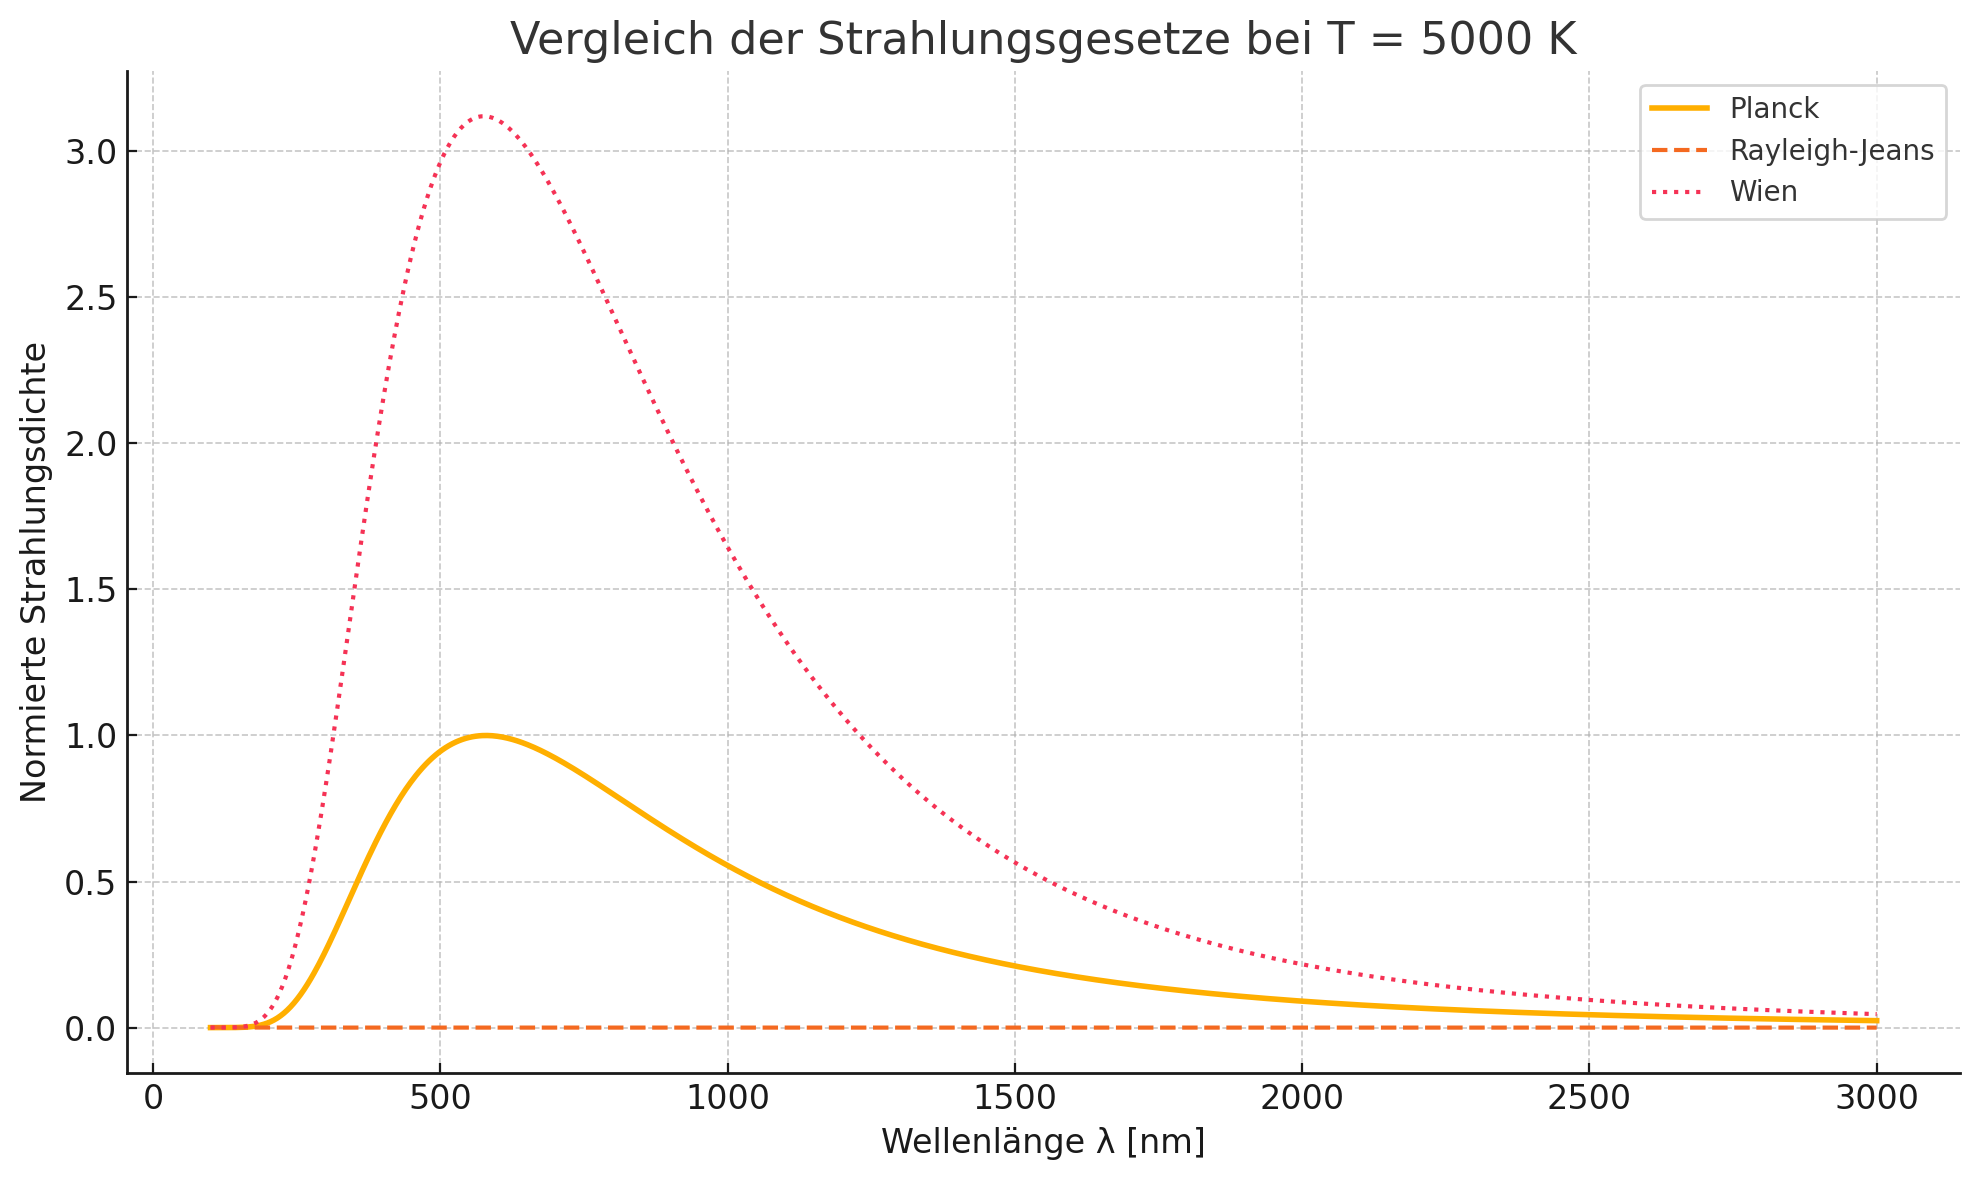
\includegraphics[width=0.85\textwidth]{bilder/strahlungsgesetze.png}
	\caption{Vergleich der drei Strahlungsgesetze. Nur das Plancksche Gesetz stimmt im gesamten Bereich mit den experimentellen Daten überein.}
	\label{fig:strahlungsgesetze}
\end{figure}

\subsubsection{Fazit}

\begin{itemize}
	\item Der Fehler der klassischen Theorie ist nicht nur groß, sondern katastrophal.
	\item Die Abweichung bei kurzen Wellen beträgt mehrere Größenordnungen.
	\item Nur das Plancksche Gesetz erklärt das gesamte Spektrum korrekt – durch die Quantisierung der Energie.
\end{itemize}

\subsection{Der Photoeffekt und Einsteins Lichtquant}\index{Photoeffekt}

Einstein ging 1905 weiter: Nicht nur die Energieabgabe, sondern das Licht selbst sei gequantelt. Er postulierte, dass ein Lichtquant (Photon) die Energie \( E = h\nu \) trägt.\index{Einstein, Albert} Nur wenn diese Energie größer ist als die Austrittsarbeit \( A \), kann ein Elektron emittiert werden:  
\[
E_{\text{kin}} = h\nu - A
\]
Dies erklärt experimentelle Beobachtungen, die mit der Wellentheorie nicht vereinbar sind – etwa die Frequenzabhängigkeit der Elektronenenergie.\index{Austrittsarbeit}

\begin{tcolorbox}[physikbox, title={Einstein (1905)\cite{einstein_lichtquanten}}]
	\label{box:einstein-lichtquant}
	„Die Entstehung von Licht erfolgt nicht überall auf der Wellenfront gleichmäßig, sondern nur an bestimmten Orten, an einzelnen Punkten.“\
	
	
	\textbf{Kommentar:} Einstein beschreibt hier bereits die Quantelung von Licht – der Startpunkt der Photonentheorie.
\end{tcolorbox}
\vspace{1em}
\index{Lichtquantenhypothese}
(Eine detaillierte Herleitung der Photoeffekt-Gleichung findet sich in Anhang~A, Abschnitt~\ref{anhangA:photoeffekt}.)
\subsection{Erste Reaktionen und Bedeutung}

Die Vorstellung, dass Licht nicht nur Wellen- sondern auch Teilcheneigenschaften besitzt, war für viele Physiker zu Beginn des 20. Jahrhunderts schwer akzeptabel. Die Wellentheorie des Lichts war durch Interferenz- und Beugungsexperimente sowie Maxwells Elektrodynamik scheinbar vollständig bestätigt.\index{Wellentheorie des Lichts} Albert Einsteins Lichtquantentheorie von 1905 – die radikale These, dass Licht aus diskreten Energiepaketen (später \emph{Photonen} genannt) besteht – widersprach dieser etablierten Sichtweise.

Einstein selbst war sich der Sprengkraft seiner Hypothese bewusst und nannte sie einen „heuristischen Gesichtspunkt“. Doch das Konzept war mehr als nur ein Rechenkniff – es erklärte den photoelektrischen Effekt vollständig und führte zu präzisen, experimentell überprüfbaren Vorhersagen.

Ein bemerkenswertes Beispiel für die anfängliche Skepsis war Robert A. Millikan.\index{Millikan, Robert A.} Obwohl er selbst 1916 in einer Reihe von Experimenten die Energieformel \( E = h \nu \) mit hoher Genauigkeit bestätigte, blieb er dem Konzept des Lichtquants lange kritisch gegenüber:

Erst nach Jahrzehnten setzte sich die Lichtquantenhypothese als fundamentaler Bestandteil der Quantenphysik durch – insbesondere nachdem auch Phänomene wie die \emph{Compton-Streuung} (1923) die Impulsnatur des Photons bestätigten.\index{Compton-Streuung}
\newpage
\noindent
Die Einführung des Photons revolutionierte nicht nur die Optik, sondern war auch entscheidend für:
\begin{itemize}
	\item die Entwicklung der \emph{Quantenmechanik},\index{Quantenmechanik}
	\item das Verständnis von \emph{Atomen und Molekülen},\index{Atom}\index{Molekül}
	\item die Theorie der \emph{Quantenelektrodynamik (QED)},\index{Quantenelektrodynamik (QED)}
	\item sowie für zahlreiche \emph{technologische Anwendungen} (Laser, Photodetektoren, Solarzellen, Quantencomputer).\index{Laser}\index{Photodetektor}\index{Solarzelle}\index{Quantencomputer}
\end{itemize}

Heute ist das Photon nicht nur ein theoretisches Konstrukt, sondern ein reales, in zahllosen Experimenten nachgewiesenes und technisch nutzbares Objekt – ein \emph{Quant der elektromagnetischen Wechselwirkung}.\index{Elektromagnetische Wechselwirkung}
\vspace{1em}
\begin{tcolorbox}[physikbox, title=Robert A. Millikan über Einstein (1916) \cite{millikan_1916}]
	\label{box:millikan-einstein}
	\emph{„Einstein’s photoelectric equation … cannot in my judgment be looked upon at present as resting upon a satisfactory theoretical foundation.“}
	
	\vspace{6pt}
	\textbf{Kommentar:} Trotz seiner experimentellen Bestätigung von Einsteins Formel lehnte Millikan das Konzept des Lichtquants zunächst ab – ein eindrucksvolles Beispiel dafür, wie tief verwurzelte theoretische Überzeugungen selbst durch klare experimentelle Befunde nicht sofort überwunden werden.
\end{tcolorbox}

\subsection{Fazit}
\vspace{1em}
\begin{tcolorbox}[hypobox, title={Was wäre, wenn nicht gequantelt wäre?}]
	\label{box:hypo-keine-quanten}
	Ohne die Annahme, dass Energie nur in diskreten Portionen ($E = nhf$) aufgenommen oder abgegeben wird:\index{Quantisierung}
	\begin{itemize}
		\item Wären fundamentale Experimente wie Schwarzkörperstrahlung und Photoeffekt unerklärbar geblieben.
		\item Wäre die klassische Physik an den Widersprüchen mit der Realität gescheitert.
		\item Hätte sich kein moderner Zugang zur Wechselwirkung von Licht und Materie entwickelt.
	\end{itemize}
	Die Quantelung war der erste Schritt zu einem neuen physikalischen Weltbild. Sie ist nicht optional – sondern grundlegend für das Verständnis des Photons.
\end{tcolorbox}

